\documentclass[CJK]{beamer}
\usepackage{CJKutf8}
\usepackage{beamerthemesplit}
\usetheme{Malmoe}
\useoutertheme[footline=authortitle]{miniframes}
\usepackage{amsmath}
\usepackage{amssymb}
\usepackage{graphicx}
\usepackage{color}
\usepackage{slashed}
\usepackage{simplewick}
\graphicspath{{../figures/}}
\def\be{\begin{equation}}
\def\ee{\nonumber\end{equation}}
\def\bea{\begin{eqnarray}}
\def\eea{\nonumber\end{eqnarray}}
\def\ii{{\dot{\imath}}}
\def\bch{\begin{CJK}{UTF8}{gbsn}}
\def\ech{\end{CJK}}
\def\bex{\begin{minipage}{0.3\textwidth}
\includegraphics[width=1in]{jugelizi.png}\end{minipage}\begin{minipage}{0.6\textwidth}}
\def\eex{\end{minipage}}
\def\chtitle#1{\frametitle{\bch#1\ech}}
\def\skipline{{\vskip0.1in}}
\def\skiplines{{\vskip0.2in}}
\def\lagr{{\mathcal{L}}}
\def\hamil{{\mathcal{H}}}
\def\vecv{{\mathbf{v}}}
\def\vecx{{\mathbf{x}}}
\def\veck{{\mathbf{k}}}
\def\vecp{{\mathbf{p}}}
\def\vecn{{\mathbf{n}}}
\def\vecA{{\mathbf{A}}}
\def\vecP{{\mathbf{P}}}
\def\vecsigma{{\mathbf{\sigma}}}
\def\hatJn{{\hat{J_\vecn}}}
\def\hatJx{{\hat{J_x}}}
\def\hatJy{{\hat{J_y}}}
\def\hatJz{{\hat{J_z}}}
\def\hatj#1{\hat{J_{#1}}}
\def\hatphi{{\hat{\phi}}}
\def\hatq{{\hat{q}}}
\def\hatpi{{\hat{\pi}}}
\def\vel{\upsilon}
\def\Dint{{\mathcal{D}}}
\def\adag{{\hat{a}^\dagger}}
\def\bdag{{\hat{b}^\dagger}}
\def\cdag{{\hat{c}^\dagger}}
\def\ddag{{\hat{d}^\dagger}}
\def\hata{{\hat{a}}}
\def\hatb{{\hat{b}}}
\def\hatc{{\hat{c}}}
\def\hatd{{\hat{d}}}
\def\hatN{{\hat{N}}}
\def\hatH{{\hat{H}}}
\def\hatp{{\hat{p}}}
\def\Fup{{F^{\mu\nu}}}
\def\Fdown{{F_{\mu\nu}}}
\def\newl{\nonumber \\}
\def\SIkm{\mathrm{km}}
\def\SIyr{\mathrm{yr}}
\def\SIGyr{\mathrm{Gyr}}
\def\SIeV{\mathrm{eV}}
\def\SIGeV{\mathrm{GeV}}
\def\SIm{\mathrm{m}}
\def\SIcm{\mathrm{cm}}
\def\SIJ{\mathrm{J}}
\def\SIs{\mathrm{s}}
\def\SIkg{\mathrm{kg}}
\def\SIg{\mathrm{g}}
\def\vece{\mathrm{e}}
\def\bmat#1{\left(\begin{array}{#1}}
\def\emat{\end{array}\right)}
\def\bcase#1{\left\{\begin{array}{#1}}
\def\ecase{\end{array}\right.}
\def\calM{{\mathcal{M}}}
\def\calT{{\mathcal{T}}}
\def\calR{{\mathcal{R}}}
\def\barpsi{\bar{\psi}}
\def\baru{\bar{u}}
\def\barv{\bar{\upsilon}}
\def\bmini#1{\begin{minipage}{#1\textwidth}}
\def\emini{\end{minipage}}
\def\qeq{\stackrel{?}{=}}
\def\torder#1{\mathcal{T}\left(#1\right)}
\def\rorder#1{\mathcal{R}\left(#1\right)}


\title{Quantum Field Theory I \\ Homework 8 solution}
  \author{}
  \date{}


\begin{document}

\begin{frame}
 
\begin{center}
\begin{Large}
\bch
量子场论 I 

{\vskip 0.3in}

第八次课后作业参考答案
\skipline
\skipline

如发现参考答案有错误请不吝告知(微信zhiqihuang或邮箱huangzhq25@sysu.edu.cn)
\ech
\end{Large}
\end{center}

\vskip 0.2in

\bch
课件下载
\ech
https://github.com/zqhuang/SYSU\_QFTI

\end{frame}

\begin{frame}
\chtitle{第1题 题目和解答}
\bch
{\small
在自然单位制下,牛顿引力常数的量纲是质量量纲的多少次方?

\skipline

解答:$G$是质量量纲的$-2$次方。(思考过程:利用万有引力公式$F = Gm_1m_2/r^2$,以及牛顿第二定律$F=m a$。)
}

\ech
\end{frame}

\begin{frame}
\chtitle{第2题 题目和解答}
\bch
{\small
以复标量场和$U(1)$规范场为例说明什么是定域规范变换不变性。

\skipline

解答:复标量场和$U(1)$规范场的拉氏密度
$$\lagr = D^\mu\phi D_\mu\phi -m^2\phi^\dagger\phi - \frac{1}{4}\Fup\Fdown$$
在规范变换
$$\phi \rightarrow \phi e^{\ii \gamma}, A_\mu \rightarrow A_\mu - \frac{1}{q}\partial_\mu \gamma$$
下保持不变。(说作用量保持不变也对)
}
\ech
\end{frame}

\begin{frame}
\chtitle{第3题 题目和解答}
\bch
{\small
简要解释如何从自由场量子化的表达式中直接读出入射和出射粒子的外线的Feynman规则。

\skipline

解答:在自由场的量子化表达式中,对入射粒子读取相应动量的湮灭算符前的系数,对出射粒子读取相应动量的产生算符前的系数。但略去体积因子和平面波函数$e^{\pm \ii kx}$。
}
\ech
\end{frame}


\begin{frame}
\chtitle{第4题 题目和解答}
\bch
{\small
设某独立系统的哈密顿算符$\hat{H}$可以写成两项之和
$$\hat{H} = \hat{H}_1 + \hat{H}_2$$


取薛定谔绘景,证明:在很短时间$dt$内,系统波函数$|\psi\rangle$的演化$e^{-\ii \hatH dt} |\psi\rangle$用下式leapfrog近似
$$ e^{-\ii \hatH dt} |\psi \rangle  \approx e^{-\ii \hatH_1 dt/2}e^{-\ii \hatH_2 dt}e^{-\ii \hatH_1 dt/2} | \psi \rangle $$
的误差为$O(dt^3)$的量级。

\skipline
解答:把两边展开到$dt^2$项比较即可证明。(具体展开式略。)
}


\ech
\end{frame}


\begin{frame}
\chtitle{第5题 题目}
\bch
{\small
课上我们学习了自由复标量场的量子化表达式
$$\hatphi_{\rm free}(x) = \frac{1}{(2\pi)^{3/2}} \int \sqrt{\frac{d^3\veck}{2\omega}} \left(\hata_{\veck} e^{-ik_\mu x^\mu} + \bdag_{\veck}e^{ik_\mu x^\mu}\right) $$

现在考虑一个有自相互作用的复标量场
$$ \lagr = \partial^\mu\phi^\dagger \partial_\mu \phi - m^2\phi^\dagger\phi - \frac{\lambda}{4}\left(\phi^\dagger\phi\right)^2$$
这里$0<\lambda\ll 1$。我们已经知道复标量场有$a$, $b$两种粒子互为反粒子。动量为$p_1$的$a$粒子和动量为$p_2$的$b$粒子发生散射变为动量为$p_3$的$a$粒子和动量为$p_4$的$b$粒子。仅考虑最低阶近似,用实线表示$a$粒子,用波浪线代表$b$粒子,请画出Feynman图并求出散射振幅。

}
\ech
\end{frame}


\begin{frame}
\chtitle{第5题 解答}
\bch
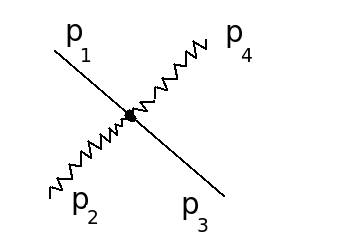
\includegraphics[width=2in]{feynman5_twosca.png}

从两个$\phi$中可以提取出$b$的产生算符和$a$的湮灭算符(交换可以得到因子2)。从两个$\phi^\dagger$中可以提取出$b$的湮灭算符和$a$的产生算符(交换可以得到因子2),从而恰好和相互作用项中的$\frac{1}{4}$抵消。结果得到:
$$\calM  = \frac{-\ii \lambda}{4\sqrt{\omega_1\omega_2\omega_3\omega_4}}$$
\ech
\end{frame}

\end{document}
